\section{Security Model}

The BioBankCloud environment deploys strong security features for concerns such as Confidentiality, Integrity and Non-repudiation ~\cite{BBCSEC} of data access. This includes authentication, authorization
, and auditing. The system allows defining different roles with different access privileges. In designing the system, we applied the Cloud Privacy Threat Modeling~\cite {CPTM} approach to identify the privacy requirements of processing sensitive biomedical data.


Figure \ref{fig:security} shows the different components of the employed security mechanisms. All BioBankCloud services are protected behind the firewall and only accessible through the secure interfaces over HTTPS channels.


\begin{figure}[h]
\centering
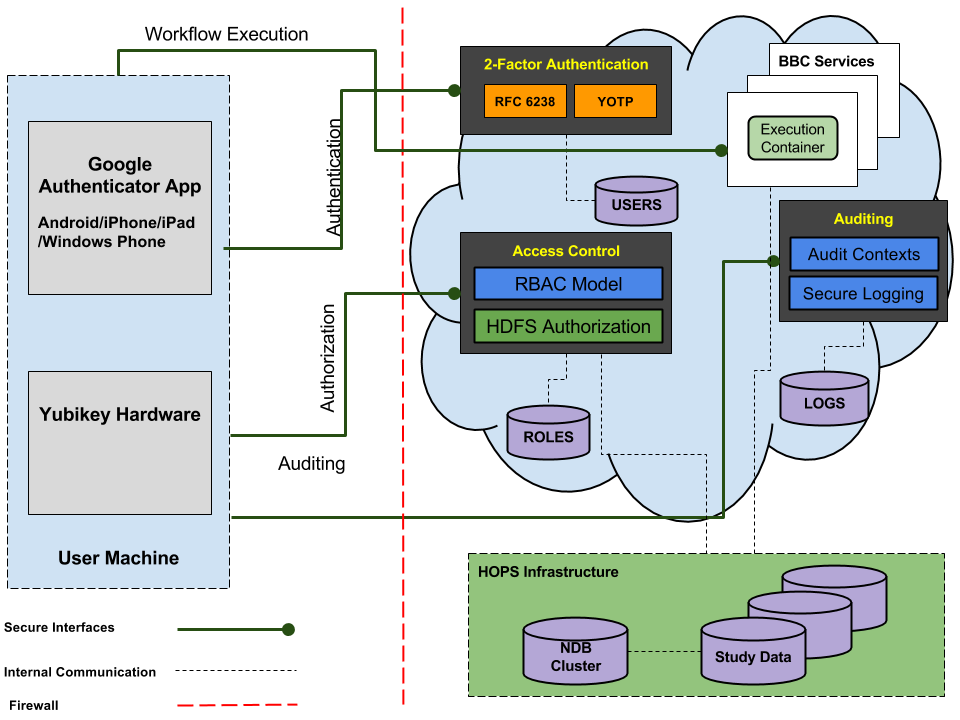
\includegraphics[width=\textwidth]{./imgs/security.png}
% stack.eps: 0x0 pixel, 300dpi, 0.00x0.00 cm, bb=0 -1 805 312                                                                                                                                               
\caption{Security Architecture of the BiobankCloud}
\label{fig:security}
\end{figure}


\subsection{2-Factor Authentication}
The authentication services map the person accessing the platform to a user identity. We provide 2-factor authentication using smart mobile devices or Yubikey \footnote {Yubikey Manual,http://www.yubico.com} hardware tokens to support different groups of users. Users send authentication requests via a Web browser to the authentication service that runs instances of the time-based one-time password (TOTP) and Yubikey one-time password (YOTP) protocols.

\subsubsection {Mobile Authentication}
The mobile user supplies an one-time generated password by the Google Authenticator \footnote{Google Authenticator, https://code.google.com/p/google-authenticator/} in addition to a simple password that was decided during the account registration. The login page authenticates the user to to the platform using the TOTP module as an implementation of the RFC 6238 \footnote{Time-Based One-Time Password (TOTP), http://tools.ietf.org/html/rfc6238}.   

\subsubsection {Yubikey Authentication}
The Yubikey enters the Yubikey device into a USB port. The user enters the simple password that was decied during the account registration and pushes the Yubikey button. The Yubikey login page authenticates the user to the platform via the YOTP module.

\subsection {Access Control}
The accessc control component ensures authorized access to genomics data as internal objects or different services within the platform. This is accomplished through a role-based access control (RBAC) model and authorization of data access on the HDFS, for example, a data owner adds/revokes members to a study and assigns privileges to access the study.

\subsection {Role-Based Access Control}

The proposed RBAC model contains information about the roles of individuals within the organization and the associated levels of access to services.

\begin{itemize}
\item Administrator: group of users who acts as the platform manager and Ethics Board.

\item Auditor: group of users with access to audit trails for auditing.

\item Data Provider: group of users who create studies, upload data and assign members to studies.

\item Guest: general visitors to the platform who are able to request an account to use the services.

\item Researcher: users of the platform that can join a study to run workflows. Researchers also can become data providers through creating a new study and uploading data to the platform.

\end{itemize}


\subsection{HDFS Supported Authorization}

\begin{figure}[h]
 \centering
 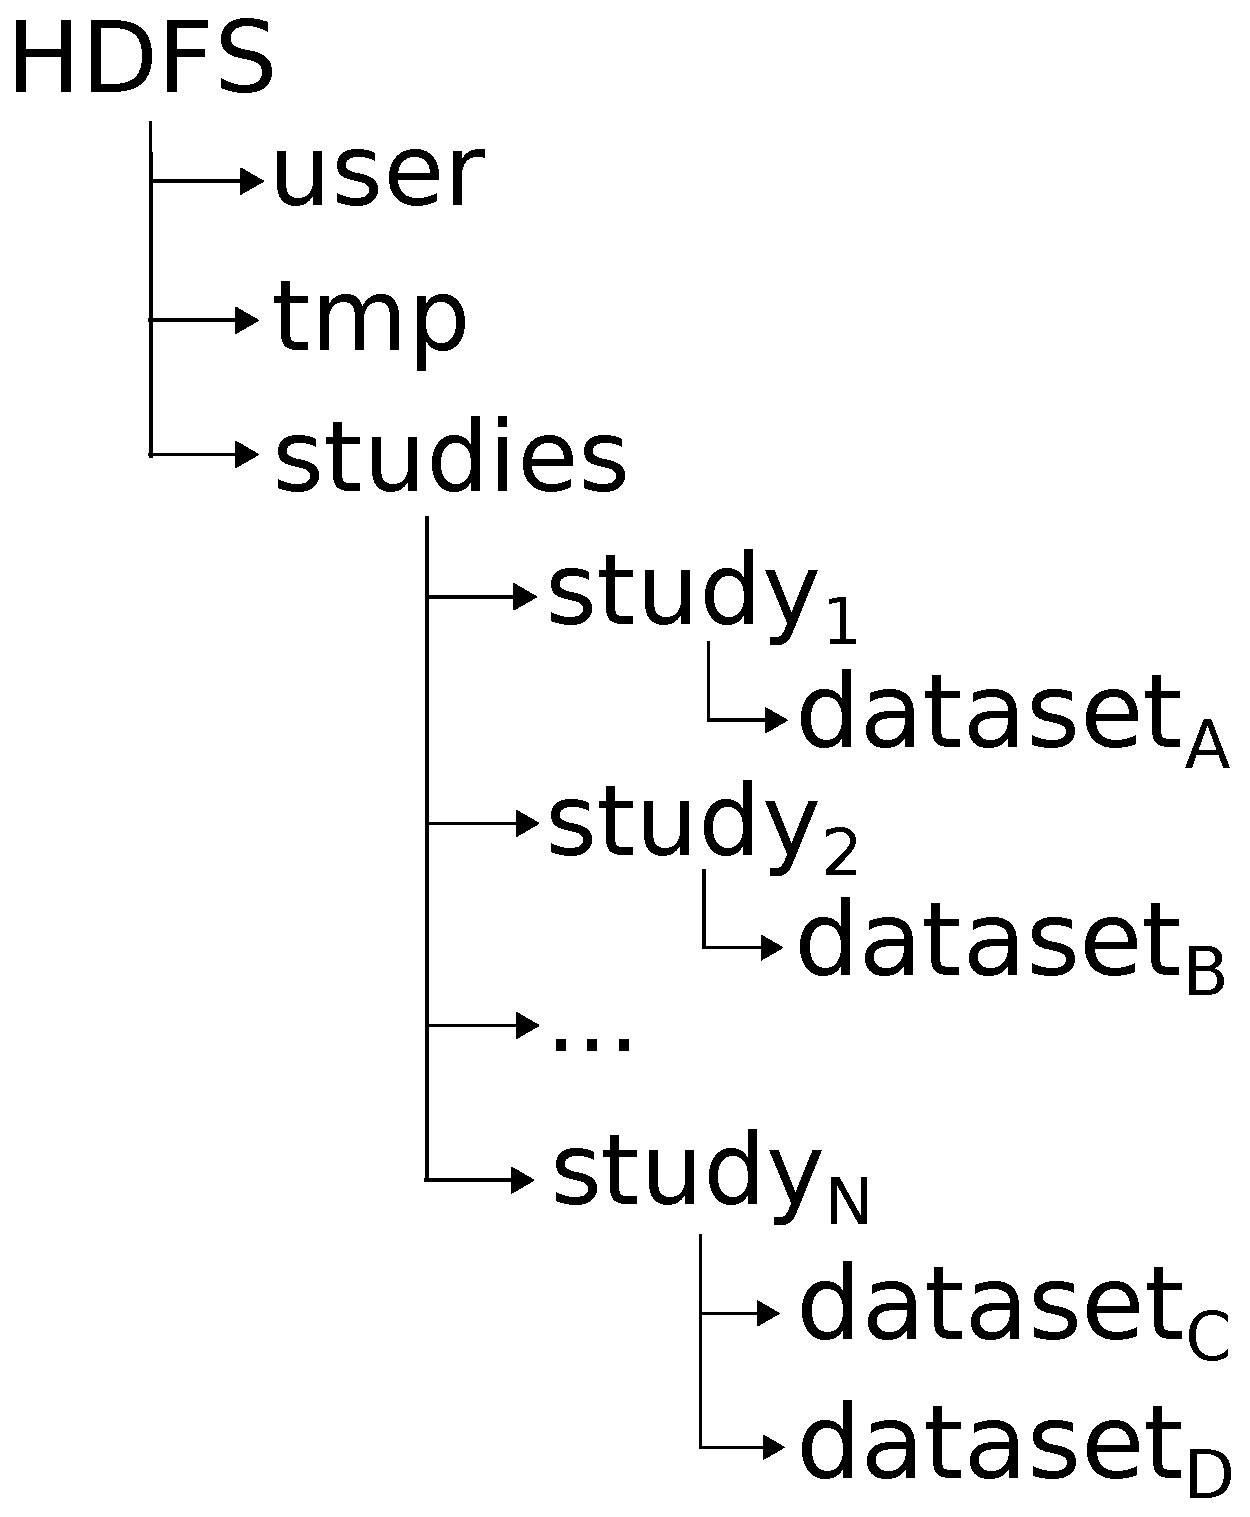
\includegraphics[scale=0.2]{./imgs/HDFS-structure.eps}
 % HDFS-structure.eps: 0x0 pixel, 300dpi, 0.00x0.00 cm, bb=0 -1 584 711
 \caption{Filesystem structure in HDFS containing Studies and DataSets.}
\end{figure}


\subsection {Auditing Service}
Finally, the auditing service enables the platform administrator or an external auditor to discover the history of accessing the platform to detect any violation to a policy. It includes several contexts \
such as role, account, study, and login audits. The secure login service assures that actions that are taken by the users are registered for tracing and auditing purposes. Each log event contains informat\
ion such as initiator, target, IP/MAC addresses, timestamp, action, and outcome.
